\section{Variations of Subgraph Isomorphism Problems}
\label{sec:apps}

So far we have discussed the basic framework of the algorithm. We have also
discussed how to compute the total number of subgraph embeddings in Algorithm
~\ref{alg:sum-reducer}. We now discuss a set of
problems that are closely related with the subgraph isomorphism problem,
including finding supervised motif and computing graphlet frequency
distribution, which can be computed using our framework.

Note that our algorithm is specifically suitable for computing on multiple
templates if they have common sub-templates, since those common sub-templates
only need to be computed once. This is the case in many problems, where
common sub-templates such as single node, edge, or simple paths are shared.

\subsection{Supervised Motif Finding}

Motifs of a real-world network are specific templates whose embeddings
occur with much higher frequencies than in random networks and are referred
as building blocks for networks. They have been found in many real-world
networks\cite{milo2002network}. Our algorithm can reduce the computational
cost for a group of templates since the common sub-templates are only computed
once, therefore is amenable to be applied in supervised motif finding. 

\iffalse
Figure
~\ref{fig:unlabel-gtree} shows the sub-templates' dependency network of a group
of unlabeled subgraphs. 

\begin{figure}[htbp]

\centerline{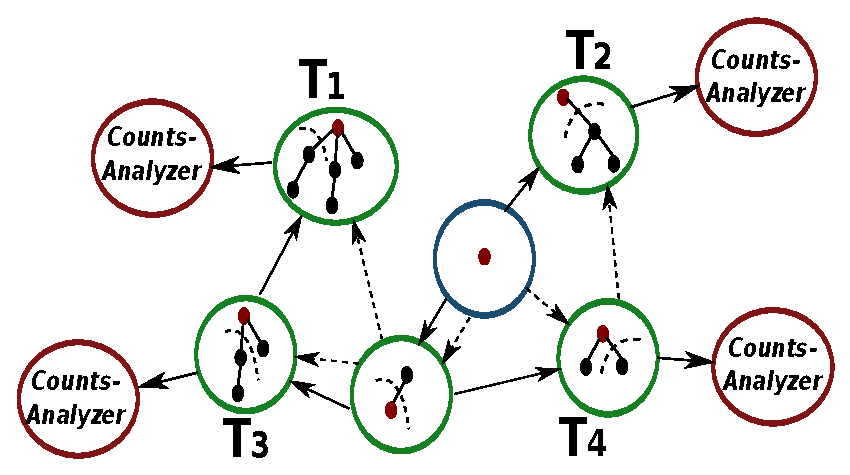
\includegraphics[width=0.35\textwidth]{plots/unlabeledGTree.eps}}

\caption{Here shows the dependency network for a group of templates from which
we want to find the motif. We can obtain the counts of the embeddings of
$T_1,\ldots,T_4$ in network $G$ and a comparable random network. By comparing
the counts of a template's embeddings in $G$ to the random network, we are able
to find the motif that has significant higher counts in $G$.}

\label{fig:unlabel-gtree}
\end{figure}

\fi

\subsection{Graphlet Frequency Distribution}
\label{sec:graphlet}

Graphlet frequency distribution has been proposed as
a way of measuring the similarity of
protein-protein networks~\cite{przulj2007biological}, where common properties
such as degree distribution, diameter, etc., may not suffice.
Unlike ``motifs'', graphlet frequency distribution is computed on all
selected small subgraphs regardless of whether they appear frequently or not.

Graphlet frequency distribution $D(i,T)$ measures the number of nodes from
which $i$ graphlets that are isomorphic to $T$ are touched on. The number of
graphlet touched on a single node $v$ can be computed using a number of counts
of the same templates $T$ with root placed at different nodes of $T$. 

\iffalse
$C(v,T(\rho_1),S), C(v,T(\rho_2),S),\ldots, C(v,T(\rho_i),S)$. E.g., in Figure
~\ref{fig:graphlet}, the graphlet frequency distribution of template 5-1 is
computed by aggregating the counts of templates 5-1-1, 5-1-2, and 5-1-3.

\begin{figure}[htbp]
\centerline{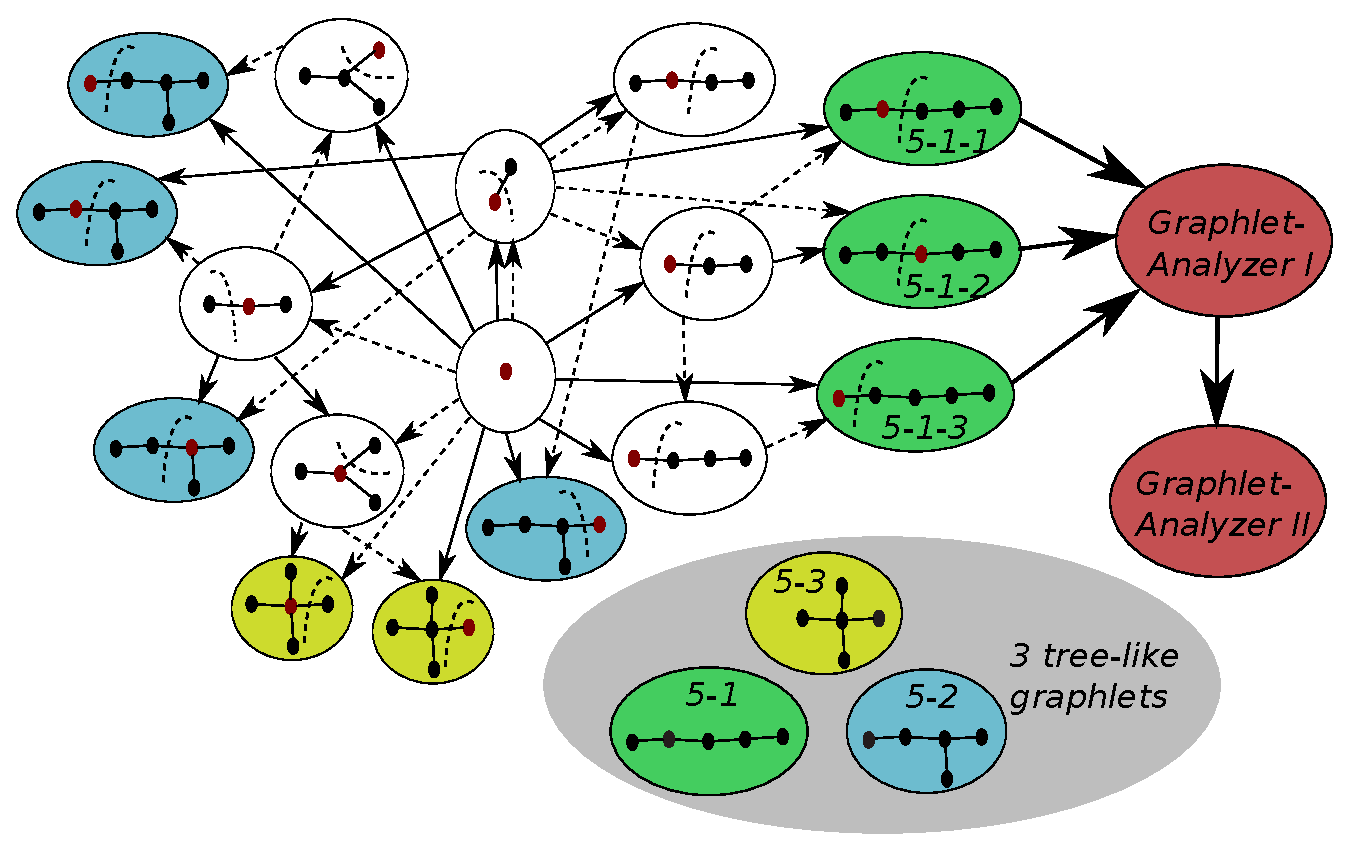
\includegraphics[width=0.45\textwidth]{plots/graphlet.eps}}

\caption{Here shows all the sub-templates needed for computing graphlet
frequency distribution on template 5-1, 5-2 and 5-3. E.g., for template 5-1,
one needs to obtain the counts $C(v, T(\rho), S_T)$ chosen multiple $\rho$s,
denoted as 5-1-1, 5-1-2 and 5-1-3. The root of a subgraph is marked red.}

\label{fig:graphlet}
\end{figure}
\fi

\iffalse

Algorithm~\ref{alg:graphlet-mapper1} to
~\ref{alg:graphlet-reducer2} show the mappers and reducers for the two jobs
corresponding to computing graphlet frequency distribution.

\begin{algorithm}[ht]
 \caption{\emph{Graphlet-AnalyzerI.Mapper(line)}}
 \label{alg:graphlet-mapper1}
\begin{algorithmic}[1]
 \STATE {$T\leftarrow GetTemplateName(line)$}
 \STATE {$P = \frac{k_i! {k \choose k_i}}{k^{k_i}}$}
 \STATE {$(v, X_{T,v}, N(v)) \leftarrow Parse(line)$}
 \STATE {$count \leftarrow 0$}
 \FOR {$\forall (s,c) \in X_{T,v}$}
 \STATE {$count = count + c$}
 \ENDFOR
 \STATE {$count = \frac{count}{P}$}
 \STATE {$Collect(\underline{key \leftarrow v},
  \underline{value \leftarrow count})$}
\end{algorithmic}
\end{algorithm}

\begin{algorithm}[ht]
 \caption{\emph{Graphlet-AnalyzerI.Reducer(key, values)}}
 \label{alg:graphlet-reducer1}
\begin{algorithmic}[1]
 \STATE {$count \leftarrow 0$}
 \FOR {$\forall value \in values$}
 \STATE {$count = count + value$}
 \ENDFOR
 \STATE {$Collect(\underline{key \leftarrow v},
  \underline{value \leftarrow count})$}
\end{algorithmic}
\end{algorithm}

\begin{algorithm}[ht]
 \caption{\emph{Graphlet-AnalyzerII.Mapper(line)}}
 \label{alg:graphlet-mapper2}
\begin{algorithmic}[1]
 \STATE {$(v, count) \leftarrow Parse(line)$}
 \STATE {$Collect(\underline{key \leftarrow count},
  \underline{value \leftarrow 1})$}
\end{algorithmic}
\end{algorithm}

\begin{algorithm}[ht]
 \caption{\emph{Graphlet-AnalyzerII.Reducer(key, values)}}
 \label{alg:graphlet-reducer2}
\begin{algorithmic}[1]
 \STATE {$freq \leftarrow 0$}
 \FOR {$\forall value \in values$}
 \STATE {$freq = freq + 1$}
 \ENDFOR

 \STATE {$Collect(\underline{key \leftarrow key},
  \underline{value \leftarrow freq})$}

\end{algorithmic}
\end{algorithm}

\fi


